\documentclass[tikz]{standalone}
\usepackage{pgfplots}
\pgfplotsset{compat=1.15}
\usepackage{mathrsfs}
\usetikzlibrary{arrows,calc}
\usepackage{tkz-euclide}

\pagestyle{empty}

\definecolor{AngleClr}{rgb}{0,0.39215686274509803,0}
\definecolor{ShapeClr}{rgb}{0.6,0.2,0}

\begin{document}

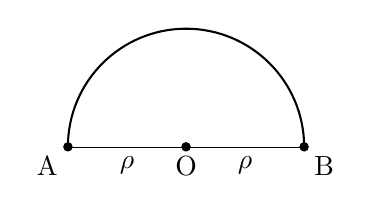
\begin{tikzpicture}[scale=.75]
\tkzSetUpLine[line width=1pt,color=black]
\tkzSetUpPoint[fill=black]

\tkzDefPoints{0/0/O,2/0/X}

\tkzDefPoint(0:2){B}
\tkzDefPoint(180:2){A}

\tkzDrawSegments[line width=0.75pt,color=black](A,B)


\tkzFillSector[fill=white](O,B)(A)
\tkzDrawArc[color=black,line width=0.75pt](O,B)(A)

\tkzDrawPoints[size=3](A,B,O)
\tkzLabelPoint[below left](A){$\rm A$}
\tkzLabelPoint[below right](B){$\rm B$}
\tkzLabelPoint[below](O){$\rm O$}

\tkzLabelSegment[below](B,O){$\rho$}
\tkzLabelSegment[below](O,A){$\rho$}

\end{tikzpicture}

\end{document}
